\newpage
\section{Diagrammes de séquence}

Le diagramme de séquence "boucle d'évenements", présente le fonctionnement du moteur de jeu. Appelé par le \textit{gameController}, l'\textit{eventLoop} va vérifier que temps s'écoule bien, et si c'est le cas, cette boucle va appeler la classe \textit{game} à exécuter un certain nombre de méthodes. Si le temps ne s'écoule pas il ne se passe absolument rien. La classe \textit{game} va parcourir chaque bâtiment et appeler certaines méthodes en fonction du type de bâtiments. Par exemple, si le bâtiment est une mine, les méthodes \textit{collectResource()}, \textit{collectMoneyOutcomes()} et \textit{consumeElectricity()}. La classe \textit{game} va alors récupérer les valeurs retournées et actualiser respectivement les ressources, l'argent et l'électricité.

\begin{figure}[H]
    \centering
    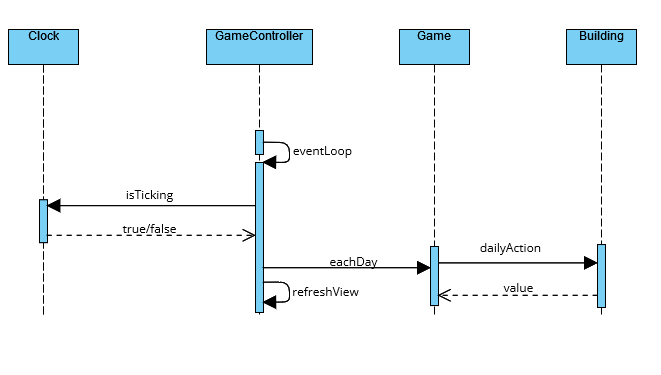
\includegraphics[width=1\linewidth]{images/eventLoop.png}
    \caption{Diagramme de séquence de la boucle d'évènement}
    \label{fig:sequenceEvent}
\end{figure}

\pagebreak

Le digramme "pose de bâtiment", présente l'enchaînement de méthodes appelées lorsqu'un joueur essaye de poser un bâtiment.

\begin{figure}[H]
    \centering
    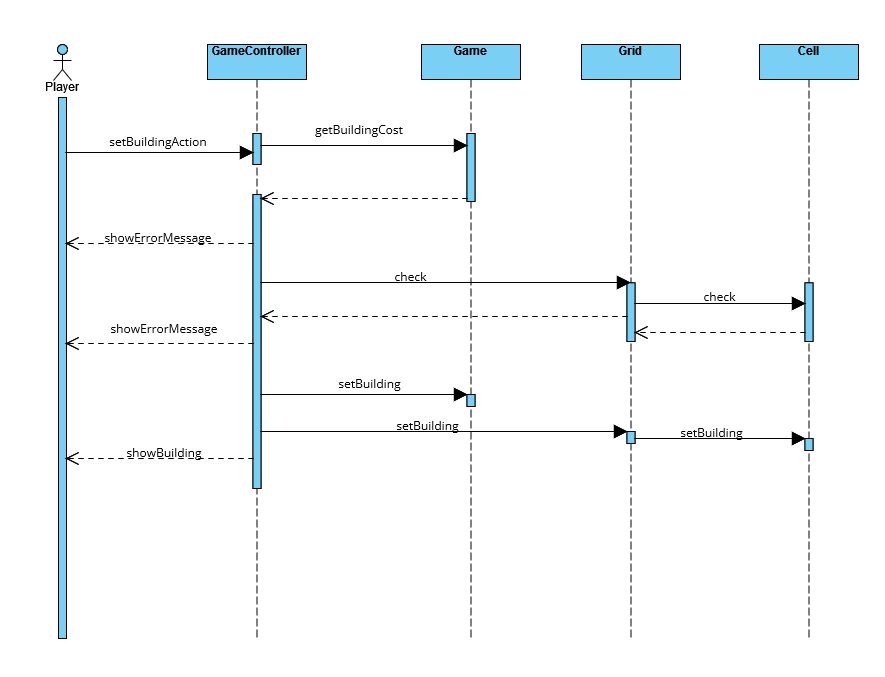
\includegraphics[width=1\linewidth]{images/setBuilding.png}
    \caption{Diagramme de séquence de la pose de bâtiment}
    \label{fig:sequenceBuilding}
\end{figure}
